\documentclass[10pt,a4paper]{report}
\usepackage[utf8]{inputenc}
\usepackage[portuguese]{babel}
\usepackage[T1]{fontenc}
\usepackage{amsmath}
\usepackage{amsfonts}
\usepackage{graphicx}
\usepackage{lmodern}
\usepackage{amssymb}
\usepackage{verbatim}
\usepackage{float}
\usepackage{minitoc}
\usepackage{hyperref}
\title{\LARGE{Introdução à Inteligência Artificial} \\ \vspace{0.5cm} \normalsize{Resumo}}
\date{}
\renewcommand{\mtctitle}{Conteúdos}

\begin{document}
\maketitle
\tableofcontents

\chapter{Procura}
\section{Formulação}
Um problema de procura pode ser formulado formalmente ao serem definidos as seguintes características:
\begin{itemize}
\item Estado
\item Estado inicial
\item Ações possíveis, dado um estado
\item Resultado de cada ação, aplicada a um estado
\item Teste do objetivo, dado um estado
\item Custo de uma ação
\end{itemize}
Em alguns tipos de problema pode-se ainda usar o $utility$, que representa o ganho ao terminar num dado estado.
\subsection{Estrutura do Espaço de Estados}
\subsubsection{Grafo}
Na representação em grafo são memorizados os estados já atingidos, pelo que precisa de mais memória, mas tem como vantagem a inexistência de ciclos infinitos
\subsubsection{Árvore}
Por oposição ao grafo, na estrutura em árvore não é necessário memorizar todos os estados já atingidos, poupando memória, mas tem como desvantagem a possível existência de ciclos infinitos
\begin{figure}[H]
\centering
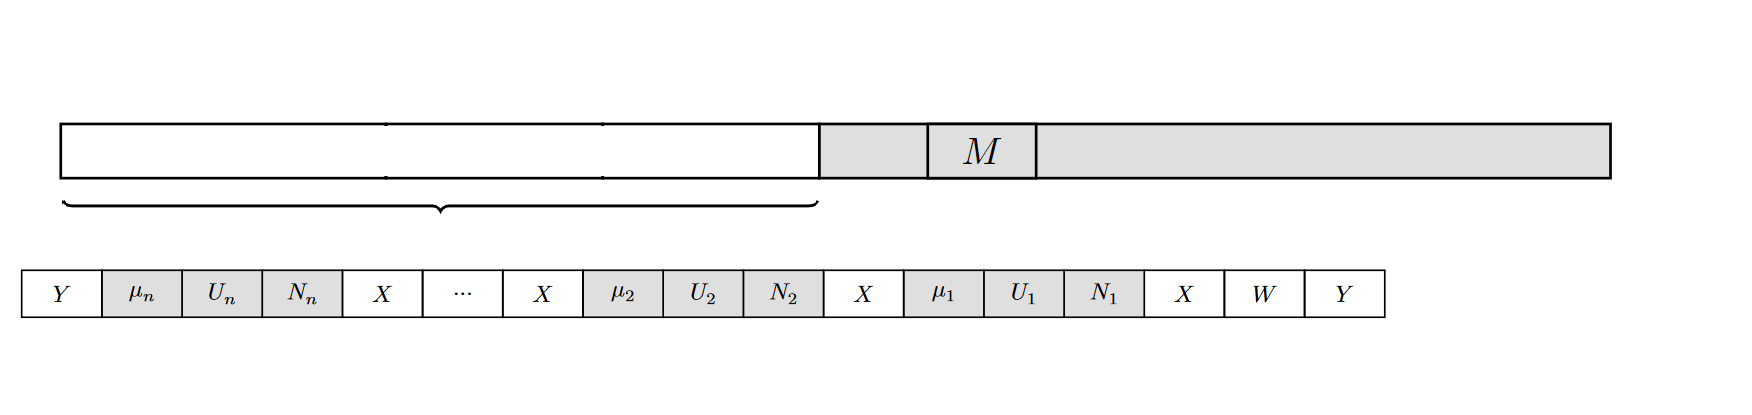
\includegraphics[scale=0.4]{Sem título.png}
\end{figure}
Os nós têm como componentes o estado, o nó ascendente, a ação aplicada a este e o custo total. A estrutura de dados na fronteira é uma fila, que pode ser do tipo FIFO, LIFO, ou priorizada.
\section{Algoritmos de Procura}
Todos os algoritmos de procura têm a mesma estrutura base:
\begin{itemize}
\item Forma-se uma árvore de procura com o estado inicial como único nó
\item Expandem-se um ou mais nós na fronteira
\item Repete-se até atingir o objetivo, ou até ter expandido todo o grafo
\end{itemize}
Diferindo apenas na escolha dos nós a expandir.
\begin{figure}[H]
\centering
\includegraphics[scale=0.5]{Sem título1.png}
\end{figure}
\subsection{Desempenho do Algoritmo}
O desempenho de um algoritmo pode ser classificado nos seguintes parâmetros:
\begin{itemize}
\item Completude - garantia de encontrar uma solução, caso exista
\item Otimalidade - garantia de encontrar a solução ótima
\item Complexidade temporal - tempo que demora a encontrar a solução
\item Complexidade espacial - memória necessária para encontrar a solução
\end{itemize}
\subsubsection{Complexidade da Procura}
A complexidade de um algoritmo tem em conta os seguintes fatores:
\begin{itemize}
\item[$b$] - Fator de ramificação 
\item[$d$] - Profundidade do objetivo mais próximo da raiz
\item[$m$] - Comprimento máximo de um caminho no espaço de estados
\end{itemize}
Sendo que a complexidade temporal corresponde, aproximadamente, ao total de nós expandidos e a espacial, ao número máximo de nós em memória.
\section{Procura Não Informada}
Na procura não informada não existe nenhuma informação sobre o que falta até ao objetivo. A procura começa no nó inicial, e expande nós da fronteira até chegar ao objetivo, falhar, ou ilimitadamente.\\
\\
Em geral, a procura não informada não consegue resolver problemas de procura de complexidade exponencial, a não ser em pequenas instâncias
\subsection{Procura em Largura}
\begin{enumerate}
\item Fronteira $\leftarrow$ estado inicial
\item Expandir todos os sucessores da fronteira
\item Fronteira $\leftarrow$ novos nós obtidos em 2.
\item Repetir desde 2.
\end{enumerate}
Este algoritmo usa uma fila FIFO e descarta novos nós que já existem, na fronteira ou expandidos. Em termos de desempenho, é completo desde que a profundidade e $b$ sejam finitos, mas não garante o caminho ótimo, apenas o objetivo mais superficial (ótimo se as ações tiverem custo uniforme). Com objetivo na profundidade $d$, a sua complexidade temporal é $O(b^d)$ (ou $O(b^{d+1})$ se o teste de objetivo for aplicado apenas ao expandir) e a sua complexidade espacial é $O(b^{d-1})$ no conjunto explorado e $O(b^d)$ na fronteira, sendo $O(b^d)$ no total.
\subsection{Procura de Custo Uniforme}
Na procura de custo uniforme expande-se o nó $n$ com menor custo acumulado $g(n)$, pelo que a fronteira é uma fila de prioridade ordenada por $g$. O teste de objetivo é aplicado quando se expande o nó.\\
\\
Este algoritmo é ótimo e completo se todos os custos > 0. A complexidade temporal e espacial é:
$$
O(b^{1+\lfloor C^*/\epsilon\rfloor})
$$
Onde $C^*$ é o custo do percurso ótimo e $\epsilon$ o custo mínimo de uma ação. Pode ser muito maior que $b^d$ se $\epsilon$ for pequeno
\subsection{Procura em Profundidade}
A procura em profundidade explora primeiro o nó mais profundo da fronteira. Usa uma fila LIFO com uma implementação recursiva. \\
\\
Este algoritmo não garante solução, podendo aprofundar indefinidamente e não é ótimo, pois devolve a primeira solução que encontrar. Seja $m$ a profundidade máxima da árvore de procura. A sua complexidade temporal é $O(b^m)$ e espacial é $O(bm)$. Existe uma variante com retrocesso em que só se expande 1 descendente de cada vez, com complexidade espacial $O(m)$.
\subsection{Aprofundamento Progressivo}
O aprofundamento progressivo faz sucessivas procuras em profundidade limitada, aumentando o limite após cada procura sem sucesso.\\
\\
Em termos de desempenho, combina as vantagens da procura em largura e profundidade. É ótimo e completo, apresentando complexidade $O(bd)$.
\subsection{Procura Bidirecional}
Na procura bidirecional, a procura faz-se em dois sentidos simultaneamente, começando na raiz em direção ao objetivo e do objetivo para a raiz.\\
\\
A complexidade reduz-se para $O(b^{d/2})$, mas ainda assim os requisitos de espaço podem ser grandes. Tem de existir uma função simples para obter os predecessores.
\section{Heurísticas}
% falar sobre admissibilidade e consistencia
Uma heurística define-se como sendo uma forma de resolver ou aproximar da resposta de um problema, sem garantias de que essa solução será ótima, perfeita ou racional.
\subsection{Classificação de uma Heurística}
Uma heurística pode ser classificada nos seguintes critérios:
\begin{itemize}
\item Admissibilidade: é admissível se é sempre não negativa e nunca sobrestima o custo de atingir o objetivo (ex. distância em linha reta)
\item Consistência: é consistente se é admissível e se dados nós $n$ e $n'$ e uma ação $a$ de $n$ para $n'$, a estimativa em $n$ não pode exceder a estimativa em $n'$ somada ao custo de $a$.
\end{itemize}
\subsection{Qualidade de uma Heurística}
Dada uma heurística, uma medida de qualidade é o seu fator de ramificação efetivo, $b*$.\\
\\
Para obter uma boa heurística por vezes é necessário relaxar as restrições do problema. Por vezes é útil começar com uma heurística inadmissível e corrigi-la. Dadas várias heurísticas $h_1, ..., h_m$ admissíveis e consistentes é possível criar uma que usa todas:
$$
h(n) = max \{h_1(n), ..., h_m(n)\}
$$
\section{Procura Informada}
A procura informada usa informação adiciona, além da especificação do problema. Usa uma função $f(n)$, de avaliação do estado e geralmente inclui uma componente heurística, onde $h(n)$ é o custo estimado de $n$ ao objetivo e $h(objetivo) = 0$.
\subsection{Procura Sôfrega (Greedy Best-First)}
Este tipo de procura usa apenas a estimativa de custo ao objetivo:
$$
f(n) = h(n)
$$
Expandindo o nó com menor $h(n)$.
\subsection{Procura $A^*$}
$A^*$ escolhe o nó com base no custo do inicio até ao nó atual e o custo do nó atual até ao objetivo:
$$
f(n) = g(n) + h(n)
$$
Ou seja, $f(n)$ é o custo estimado da melhor solução que passa por $n$. $A^*$ é completo e ótimo, desde que $b$ seja finito, o custo das ações seja maior que 0 e $h(n)$ seja admissível (na procura em árvore) ou consistente (em grafo).\\
\\
Este algoritmo para quando se vai expandir o nó objetivo. Quando o nó a expandir é um objetivo garante-se que não há nenhum caminho melhor para atingir um objetivo, pelo que expande todos os nós com $f(n) < C^*$, pode expandir nós com $f(n) = C^*$ e não expande nós com $f(n) > C^*$, onde $C^*$ é o custo ótimo.\\
\\
Nenhum outro algoritmo que use a mesma heurística garante expandir menos nós. A sua complexidade é $O(b^\epsilon d)$, em que $\epsilon$ é o erro relativo da heurística, $\epsilon \equiv (h^*  - h)/h^*$ ($h^*$ é a heurística ótima) e o fator de ramificação efetivo é $b^\epsilon$.
\subsubsection{$A^*$ Ponderado}
Esta versão do $A^*$ tem o requisito de otimalidade mais relaxado, de forma a resolver melhor problemas de grande dimensão. A sua função é a seguinte:
$$
f(n) = g(n) + W \cdot h(n)
$$
Onde $W$ é um valor arbitrário.
\section{Procura Adversarial}
A procura adversarial é usada em jogos, pelo que o tempo de decisão é um fator crucial.
\subsection{Minimax}
O algoritmo minimax pretende maximizar ou minimizar o resultado final obtido. Para isso simula cada uma das jogadas possíveis e cada uma das respostas possíveis do adversário, considerando sempre o pior caso, até uma profundidade especificada:
\begin{figure}[H]
\centering
\includegraphics[scale=0.5]{Sem título2.png}
\end{figure}
O minimax faz uma pesquisa completa em profundidade, com complexidade temporal $O(b^m)$ e espacial de $O(bm)$ se expande de uma vez todas as ações de um nó ou $O(m)$ se expande à vez cada ação de um nó. Não é viável em jogos complexos.
\subsubsection{Alfa-Beta}
A poda alfa-beta é uma variante do minimax onde não se expandem caminhos que não podem influenciar o resultado.\\
\\
\begin{minipage}[c]{0.4\textwidth}
A poda pode ser feita pelo menor valor (nó MIN): se o valor de $n$ for menor do que a, não vale a pena expandir mais irmãos de $x$ e $n$ porque MAX, na jogada acima, nunca há-de escolher esse ramo
\end{minipage}\hfill
\begin{minipage}[c]{0.5\textwidth}
\begin{figure}[H]
\centering
\includegraphics[scale=0.5]{Sem título3.png}
\end{figure}
\end{minipage}
\begin{minipage}[c]{0.4\textwidth}
Ou pelo maior valor (nó MAX): se o valor de $n$ for maior do que $a$, não vale a pena expandir mais irmãos de $x$ e $n$ porque MIN, na jogada acima, nunca há-de escolher esse ramo.
\end{minipage}\hfill
\begin{minipage}[c]{0.5\textwidth}
\begin{figure}[H]
\centering
\includegraphics[scale=0.5]{Sem título4.png}
\end{figure}
\end{minipage}
\begin{itemize}
\item $\alpha$ é o valor da melhor escolha do MAX até agora
\item $\beta$ é o valor da melhor escolha do MIN até agora
\end{itemize}
\begin{figure}[H]
\centering
\includegraphics[scale=0.5]{Sem título5.png}
\end{figure}
A sua complexidade temporal é $O(b^{3m/4})$ se os sucessores estiverem por ordem aleatória e $O(b^{m/2})$ se os sucessores estiverem ordenados.
\section{Procura Adversarial Incompleta}
Na procura adversarial podem haver ações de resultado não determinista, árvores demasiado grandes para expansão completa ou outras imperfeições. Existem duas estratégias neste caso:
\begin{itemize}
\item[A] - Explora todos os lances até certa profundidade e usa uma heurística para determinar a utilidade dos estados a essa profundidade. Explora uma parte da árvore a toda a largura, mas pouco profunda.
\item[B] - Ignora lances que parecem maus e explora linhas promissoras quando possível. Explora uma parte profunda mas estreita da árvore
\end{itemize}
\subsection{Minimax Heurístico}
O minimax heurístico usa a estratégia A e recebe o estado atual $s$ e a profundidade de procura $d$. O custo do ponto de corte é estimado com a função de avaliação heurística EVAL e o teste terminal é substituído pela função CUTOFF-TEST.\\
\\
Perde-se a otimalidade e a qualidade do jogador depende muito da qualidade das heurísticas.
\subsection{Procura Monte Carlo em Árvore}
Na procura monte carlo o valor do estado é estimado pela utilidade média do resultado de vários jogos simulados, devendo se escolhida uma boa política de escolha de jogadas. Cada iteração segue os seguintes passos:
\begin{itemize}
\item Seleção sucessiva de jogadas dos dois jogadores, probabilisticamente
\item Expansão, chegado a uma folha gera um ou mais novos nós
\item Simulação a partir do novo nó gerado, escolhe lances de acordo com a política de seleção (lances não memorizados na árvore) até chegar a um desfecho
\item Retropropagação, propagando o resultado até à raiz da árvore
\end{itemize}
Uma abordagem eficiente á política de seleção é a $upper$ $confidence$ $bounds$:
$$
UCB(n) = \frac{U(n)}{N(n)} + C \cdot \sqrt{\frac{\log[N(parent(n))]}{N(n)}}
$$
Onde:
\begin{itemize}
\item $U(n)$ é o total da utilidade dos jogos que usam o nó $n$
\item $N(n)$ é o total de jogos que usam o nó $n$
\item $parent(n)$ é o nó ascendente de $n$
\item $C$ é a constante de balanço entre diversificação e aprofundamento ($\sqrt{2}$ recomendado)
\subsection{Expectiminimax}
Este algoritmo é usado em jogos estocásticos, onde as jogadas envolvem algum grau de aleatoriedade. Os nós passam a ter um valor esperado e é necessário incluir nós de acaso, alem de MIN e MAX. A sua função de avaliação tem de ser uma transformação linear da probabilidade de vencer (utilidade esperada) numa posição.\\
\\
A sua complexidade é $O(b^mn^m)$, onde $n$ é o número de eventos aleatórios possíveis em cada jogada
\end{itemize}
\section{Procura Local}
A procura local é usada em contextos não observáveis, não determinísticos ou desconhecidos. Neste caso não interessa o caminho até ao objetivo e pode não se saber se já se atingiu o ótimo.\\
\\
Este tipo de procura parte de um estado inicial (aleatório ou pré-definido) e explora estados vizinhos. A procura não é sistemática, pelo que pode não explorar a região onde está o ótimo. Tem como vantagens o uso de pouca memória e frequentemente encontra soluções razoáveis em espaços potencialmente infinitos.
\subsection{Procura em Espaços Contínuos}
Num espaço contínuo não é possível obter toda a vizinhança, pelo que é necessário discretizar o espaço ou calcular o gradiente local da função:
$$
\nabla f = \left( \frac{\partial f}{\partial x_1}, \frac{\partial f}{\partial x_2}, ..., \frac{\partial f}{\partial x_n} \right)
$$
O que permite escolher a direção que provoca a maior melhoria na definição do passo $\alpha$, $x = x + \alpha \nabla f (x)$.
\subsection{Algoritmo Trepa-Colinas}
Este algoritmo processa-se da seguinte forma:
\begin{itemize}
\item estado atual $\leftarrow$ estado inicial
\item repete
\begin{itemize}
\item novo $\leftarrow$ melhor dos vizinhos
\item se novo $\leq$ estado atual então retorna estado atual (máximo local)
\item estado atual $\leftarrow$ novo
\end{itemize}
\end{itemize}
A variante representada é a de maior subida, mas existem outras, por exemplo, com movimentos laterais, estocástico ou de reinício aleatório.\\
\\
Este algoritmo não lida bem com algumas situações, tais como a existência de máximos locais ou vizinhanças muito grandes.
\subsection{Recozimento Simulado}
Este algoritmo é o híbrido entre o trepa-colinas e o random walk, resultando num trepa-colinas que admite movimentos descendentes.
\subsection{Procura em Feixe}
A procura em feixe explora $k$ estados iniciados aleatoriamente. Para cada um dos $k$ estados gera todos os seus sucessores e seleciona os $k$ melhores até chegar a um objetivo.\\
\\
Existe uma versão estocástica onde em vez de selecionar os $k$ melhores sucessores, estes são selecionados probabilisticamente, com probabilidade proporcional á sua qualidade.
\subsection{Algoritmo Genético}
No algoritmo genético existe um conjunto de indivíduos e as soluções são sujeitas ás seguintes operações, em cada ciclo:
\begin{itemize}
\item seleção: operador não-determinista, seleciona tendencialmente os melhores indivíduos
\item sobrecruzamento: combina duas soluções para obter dois descendente
\item mutação: altera aleatoriamente (com baixa probabilidade) as caraterísticas de um indivíduo (solução)
\item substituição: produz a geração seguinte selecionando indivíduos dos descendentes e da geração anterior
\end{itemize}
A mutação é um operador opcional.

\chapter{Satisfação de Restrições}
Um problema de satisfação de restrições tem uma representação fatorizada em variáveis, onde cada uma tem um valor. O problema fica resolvido quando os valores das variáveis satisfazerem todas as restrições.
\section{Formulação}
Para formular formalmente um CSP deve-se definir:
\begin{itemize}
\item $X$: conjunto das variáveis $\{X_1,...,X_n\}$
\item $D$: conjunto dos domínios, $\{D_1,...,D_n\}$, um para cada variável
\item $C$: conjunto de restrições $\{C_1,...,C_n\}$ que especifica combinações de valores admissíveis
\end{itemize}
Onde $D_i$ é o conjunto de valores possíveis para a variável $X_i$ e $C_i = <ambito,rel>$, onde $ambito$ é um tuplo de variáveis envolvidas na restrição $i$ e $rel$ é a relação que define os valores que as variáveis podem tomar. Por exemplo, supondo duas variáveis $X_1$ e $X_2$, ambas com domínio $\{1,2,3\}$, pode-se expressar que $X_1$ tem de ser maior que $X_2$ de duas formas: A forma explícita:
$$
\langle (X_1,X_2),\{(3,1),(3,2),(2,1)\} \rangle
$$
E a forma funcional, ou implícita:
$$
\langle (X_1,X_2), X_1 > X_2 \rangle
$$
Um CSP pode-se representar sob a forma de um grafo, onde os nós representam as variáveis e os arcos representam as restrições.
\subsection{Propagação de Restrições}
É possível usar as restrições para reduzir o domínio de uma variável, o que pode reduzir o domínio de outras.\\
\\
Trata-se de um passo prévio á procura mas que pode resolver o problema, no caso de haver apenas uma ou nenhuma solução possível.\\
Um nó diz-se consistente se todos os valores do domínio da variável satisfazem as suas restrições unárias. Um arco diz-se consistente se todos os valores do domínio da variável satisfazem as suas restrições binárias.
\subsubsection{AC-3}
Este algoritmo permite obter consistência num arco:
\begin{itemize}
\item Começa com a lista de todos os arcos
\item Escolhe $(X_i,X_j)$ aleatórios e torna $X_i$ um arco consistente face a $X_j$
\begin{itemize}
\item Se $D_i$ não se altera, passa a outro arco
\item Se $D_i$ diminui, junta á lista os arcos $(X_k,X_i)$, em que $X_k$ são todos os vizinhos de $X_i$ ($D_k$ pode diminuir)
\item Se $D_i$ ficar vazio o problema não tem solução
\end{itemize}
\item Repete até a lista estar vazia
\end{itemize}
O resultado é um CSP equivalente com domínios menores.
\subsubsection{Consistência de Percurso}
$\{X_i,X_j\}$ são consistentes em percurso relativamente a $X_m$ se para cada $\{X_i=a, X_j=b\}$ consistente com as restrições de $\{X_i,X_j\}$ existir uma atribuição a $X_m$ que satisfaz as restrições de $\{X_i,X_m\}$ e $\{X_m,X_j\}$.
\subsection{Restrições de Ordem Superior}
Restrições de ordem superior têm um número arbitrário de variáveis.\\
\\
Um exemplo é o $alldiff$, onde existem $m$ variáveis e $n$ valores diferentes possíveis.
\section{Algoritmos para Resolução}
Nos casos onde existe mais que uma solução possível, a propagação de restrições não consegue resolver o problema, sendo necessário o uso de um algoritmo de procura em CSP.
\subsection{Procura com Retrocesso}
Este tipo de procura baseia-se na comutatividade do CSP. Consiste em procura em profundidade e retrocesso quando uma variável não tem valores possíveis.\\
\\
Reduz a complexidade de $O(n!d^n)$ para $O(d^n)$.
\subsection{Intercalação de Procura com Inferência}
Esta estratégia é melhor que aplicar só uma vez inferência e depois procura. Uma das suas formas mais simples consiste em verificar a consistência de arco cada vez que se escolhe um valor para uma variável.
\subsection{Melhoramento Iterativo}
O melhoramento iterativo é um método de procura local sobre estados completos, que repara iterativamente estados inconsistentes. Enquanto houver conflitos é selecionada aleatoriamente uma variável e, se tiver inconsistências, é usada uma heurística para escolher um novo valor.
\subsubsection{Min-conflitos}
Min-conflitos é uma heurística para escolher um novo valor. Consiste em escolher o valor que minimiza o número de conflitos com outras variáveis.

\chapter{Planeamento}
Em problemas de planeamento assume-se que o mundo é determinístico, o agente sabe o estado atual, o tempo é discreto e orientado por eventos e os objetivos são predicados de estados que devem ser atingidos. O planeamento consiste em encontrar uma sequência de ações para, a partir do estado inicial, atingir o objetivo.
\section{Formulação}
\subsection{Estados}
Um estado é representado por uma conjunção de predicados, objetos ou variáveis. Por exemplo:
\begin{itemize}
\item $Noite$
\item $Em(Casa,Manuel)$
\item $Aberta(Porta) \land \lnot Acesa(Luz)$
\end{itemize}
\subsection{Pré-Condições}
Uma ação instanciada $a$ é aplicável no estado $s$ se:
\begin{itemize}
\item Todos os literais afirmados na pré-condição estão em $s$
\item Todos os literais negados na pré-condição não estão em $s$
\end{itemize}
Isto é, as pré-condições de $a$ decorrem do estado $s$.
\subsection{Ações}
Ações são representadas por um esquema de ação na forma: nome; lista de variáveis; pré-condições; efeito. Por exemplo:
$$
Voar(p,de,para), pre-cond: Em(p,de) \land Aviao(p) \land Aeroporto(de) \land Aeroporto(para),
$$
$$
efeito: \lnot Em(p,de) \land Em(p,para)
$$
\subsubsection{Resultados}
O resultado de aplicar uma ação $a$ a um estado $s$ é um estado $s'$ obtido da seguinte forma:
\begin{itemize}
\item Removem-se as afirmações negativas no efeito: $Del(a)$
\item Adicionam-se as afirmações positivas no efeito: $Add(a)$
\end{itemize}
$$
s' = Result(s,a) = (s - Del(a)) \cup Add(a)
$$
\section{Heurísticas}
\subsection{Heurística de Ignorar Pré-Condições}
Nesta heurística relaxa-se o problema, assumindo que todas as ações se podem aplicar a todos os estados.\\
\\
Mais precisamente, removem-se todas as pré-condições das ações e todos os efeitos exceto os que são literais no objetivo e conta-se o número mínimo de ações para atingir o objetivo. Por vezes pode não ser possível ignorar todas as pré-condições, optando-se por pré-condições parciais.
\subsection{Heurística de Abstração de Estados}
Esta heurística permite reduzir muito o número de estados, mapeando vários num único. Uma solução neste espaço de estados será menor que no problema original e é posteriormente fácil alargar a solução ao problema original.
\subsection{Heurística da Decomposição}
Nesta heurística decompõe-se o objetivo em diversos. Por vezes é usada juntamente com a heurística do máximo dos subconjuntos de objetivos e com a heurística da soma dos custos dos subconjuntos. 
\section{Algoritmos de Planeamento}
\subsection{Procura Adiante}
A partir do estado inicial usam-se as ações definidas para avançar até ao objetivo. O espaço de procura cresce exponencialmente com fator de ramificação, mas podem-se derivar heurísticas fortes.
\subsection{Procura Retrógrada}
Este tipo de procura age de forma oposta á adiante. Começa no objetivo e retrocede no espaço de estados. Dado um estado $s$ e uma ação $a$ que levou a esse estado, a regressão ao estado anterior $s'$ é:
$$
s' = (s - Add(a)) \cup Pre\_cond(a)
$$
Os estados candidatos à regressão têm de ter efeitos da ação que unifiquem com os do estado a regredir, pelo menos 1 deles, e não podem ter efeitos da ação que neguem algum efeito do estado a regredir. Por exemplo, $s = B \land C \land D$ e uma ação $a$ com efeitos $B \land C \land \lnot D$ pois nesse caso $a$ não leva ao estado $s$ e seria necessária, pelo menos, mais uma ação, para lá chegar.\\
\\
É mais difícil encontrar uma boa heurística para a procura retrógrada, visto que trabalha com conjuntos de estados, por oposição á procura adiante que usa estados específicos.
\section{Planeamento com Tempo}
Em muitos casos, planos envolvem tempo, através da duração das ações e recursos, que podem ser consumíveis ou reutilizáveis.
\subsection{Ordenação de Ações}
Sendo $A$ e $B$  ações, $A \prec B$ significa que $A$ precede $B$. O modelo de calendarização é o seguinte:
$$
ES(Start) = 0
$$
$$
ES(B) = max_{A \prec B}(ES(A) + Duration(A))
$$
$$
LS(Finish) = ES(Finish)
$$
$$
LS(A) = min_{B \succ A}(LS(B) - Duration(A))
$$
\section{Planeamento Hierárquico}
O planeamento hierárquico é organizado em macro-ações, que podem ser posteriormente expandidas em planos detalhados.
\subsection{Ações de Alto Nível}
As ações de alto nível são usadas no planeamento hierárquico, sendo composições de outras ações. É possível formar um plano de alto nível com ações de alto nível. Um plano de alto nível atinge o objetivo a partir de um estado se pelo menos uma das suas implementações atinge o objetivo a partir desse estado.
\section{Planeamento em Sistemas Multi-Agente}
Quando existe mais que um agente é necessário planear vários fluxos de ações.
\subsection{Tipos de Concorrência}
\subsubsection{Execução Intercalada}
Na execução intercalada o plano tem de ser correto em qualquer possibilidade. Não são modeladas ações em simultâneo e cresce exponencialmente com agentes e ações.
\subsubsection{Ordem Parcial}
Na ordem parcial diz-se que $a_1$ tem de ocorrer antes de $a_2$, mas nada se diz entre $a_1$ e $b_1$, podendo ocorrer em simultâneo ou sequencialmente.
\subsubsection{Sincronização Perfeita}
Usa-se um relógio global, onde as ações iniciadas num instante temporal são simultâneas e demoram todas o mesmo tempo.
\subsection{Planeador Centralizado}
Um planeador centralizado planeia as ações para todos os agentes. A procura no espaço de ações tem as seguintes considerações:
\begin{itemize}
\item 1 ator: $b$ ações possíveis para $a$ em $RESULT(s,a)$
\item $n$ atores: $b^n$ ações possíveis
\end{itemize}
\subsection{Planeador Distribuído}
Num planeador distribuído cada agente planeia as suas ações. Existe sucesso de os agentes concordarem no mesmo plano, mas em diversos casos é necessário os agentes chegarem a acordo sobre um plano conjunto. Alguns protocolos para chegar a acordo são: leilão, negociação, argumentação.
\chapter{Aprendizagem Automática}
Um programa diz-se aprender de experiência $E$, com respeito a uma classe de tarefas $T$ com medida de performance $P$, se a sua performance em tarefas do tipo $T$, medida por $P$, melhora com experiência $E$.
\section{Aprendizagem Supervisionada}
Dado um conjunto de treino de $N$ exemplos $(x_1,y_1), (x_2,y_2), ..., (x_N,y_N)$ em que $x_i$ é um vetor de atributos e $y_i$  o resultado desse exemplo, dado por uma função desconhecida $y_i = f(x_i)$. Pretende-se encontrar uma função $h$ (hipótese) de aproxima $f$.\\
\\
A denominação de supervisionada ocorre pois considera-se que o resultado $y_i$ é fornecido por um "professor".
\subsection{Componentes}
Existem os atributos, que representam cada uma das características dos casos do problema. Podem ser de diversos tipos:
\begin{itemize}
\item Reais
\item Inteiros
\item Binários
\item Categóricos (ex: urbano, rural, ...)
\end{itemize}
E existe a variável de resposta, que corresponde ao contra-domínio da função que se está a aprender. Estes valores podem ser discretos ou contínuos.
\subsection{Aprendizagem Robusta}
Interessa obter resultados corretos em mais exemplos do que os usados na aprendizagem, pelo que  a avaliação da aprendizagem é feita com um outro conjunto de exemplos, conjunto de teste, distinto do conjunto de treino.
\subsection{Classificador Naïve Bayes}
O classificador naïve Bayes é um método usado frequentemente em aprendizagem supervisionada, que permite classificar um objeto a partir de um conjunto de treino, com base nas suas características. Trata-se de um modelo de probabilidade condicionada, onde dada uma classe $c$ e um conjunto de atributos $a =\{x, y, z\}$, a probabilidade de um objeto com estes atributos ser da classe $c$ é:
$$
P(c|x,y,z) = \frac{P(c)\displaystyle\prod_j(a_j|c)}{P(x,y,z)} = \alpha P(c)P(x|c)P(y|c)P(z|c)
$$
Onde $\alpha$ é uma constante obtida a partir do conjunto de treino, corresponde á percentagem de $c$'s no conjunto de treino:
$$
\alpha = \frac{1}{P(x,y,z)}
$$
Trata-se de um classificador simples mas robusto.
\section{Árvores de Decisão}
A árvore de decisão é um dos modelos mais simples e usados na aprendizagem automática. Os resultados são produzidos por uma série de testes aos valores dos atributos em cada nó, sendo que as folhas têm os resultados a retornar.
\subsection{Árvore Booleana}
Este tipo de árvore é equivalente a uma declaração lógica na forma:
$$
Resultado \Leftrightarrow (Caminho_1 \lor Caminho_2 \lor ...)
$$
Em que $Caminho_i$ é uma conjunção da forma $(A_i  = v_{i_x} \land ...)$. Qualquer função em lógica proposicional pode ser expressa sob a forma de uma árvore de decisão binária.
\begin{figure}[H]
\centering
\includegraphics[scale=0.5]{Sem Título6.png}
\end{figure}
\subsubsection{Entropia}
Uma estratégia para dividir e conquistar consiste em escolher o atributo mais importante primeiro (o que mais distingue a classificação dos exemplos) e repetir recursivamente até só haver folhas. Para determinar qual o atributo mais importante usa-se a entropia da informação, calculada sobre uma v.a. a partir da distribuição probabilística:
$$
H(X) = \sum_k P(x_k) \log \frac{1}{P(x_k)} = -\sum_k P(x_k) \log P(x_k)
$$
Usando-se $\log_2$ a unidade é o $bit$. Por exemplo, numa moeda com 99\% de probabilidade de sair cara($F$):
$$
H(F) = -(0,99\log_2 0,99 + 0,01 \log_2 0,01) \approx 0,08 \; bit
$$
Escolhendo um atributo $A$ com $d$ valores, definem-se $d$ subconjuntos, cada um deles com $p_k$ exemplos positivos e $n_k$ negativos ($p+n$ representa o número total de elementos do atributo), com entropia $B(p_k/(p_k+n_k))$. Escolhendo esse atributo a entropia restante é:
$$
HRestante(A) = \sum_k^d \frac{p_k + n_k}{p + n}B\left(\frac{p_k}{p_k+n_k}\right)
$$
Por exemplo, na árvore apresentada acima, considerando o atributo $Patrons$, com 12 elementos, a sua entropia restante seria:
$$
HRestante (Patrons) = \frac{2}{12} B\left(\frac{0}{2}\right) + \frac{4}{12} B\left(\frac{4}{4}\right) + \frac{6}{12} B\left(\frac{2}{6}\right) \approx 0,459 \; bit
$$
O ganho de entropia com a escolha do atributo $A_i$ é:
$$
GanhoH(A_i) = B \left(\frac{p}{p + n}\right) - HRestante(A_i)
$$
Onde $B$ representa a entropia de uma v.a. booleana: 
$$
B(q) = -(q\log_2 q+(1-q)\log_2 (1-q))
$$
Como se quer escolher o atributo com maior ganho, basta escolher o que produz menor $HRestante$.
\subsection{Overfitting}
Overfitting acontece quando a aprendizagem é demasiado focada nos exemplos. Em árvores de decisão pode-se realizar:
\begin{itemize}
\item poda prévia – limita a profundidade máxima da árvore, com a desvantagem do efeito horizonte
\item poda posterior – depois da árvore completa eliminam-se nós de modo a simplificar a árvore, com a desvantagem da árvore completa poder ser muito grande
\end{itemize}
\subsubsection{Poda Posterior Simples}
Começando nas folhas, cada nó é substituído pela sua classe mais frequente. Se a precisão estimada não for significativamente afetada, mantém-se a alteração.
\subsection{Validação Cruzada}
Para melhorar a identificação do ponto de paragem da aprendizagem sobre conjuntos de treino e melhor estimar o erro de generalização deve usar-se k-fold cross-validation: divide-se o conjunto de treino em $k$ subconjuntos do mesmo tamanho. Fazem-se $k$ rondas de aprendizagem, uma com cada um dos subconjuntos para validação.
\begin{figure}[H]
\centering
\includegraphics[scale=0.5]{Sem Título7.png}
\end{figure}
Vai-se verificando o erro médio nos subconjuntos de validação e quando este atinge o mínimo, é o bom ponto de paragem.
\section{Vizinhos mais Próximos}
\subsection{Distâncias}
Distância Euclideana:
$$
D(x_j,x_q) = \sqrt{\sum_i(x_{ji} - x_{qi})^2}
$$
Distância de Manhattan:
$$
D(x_j,x_q) = \sum_i|x_{ji} - x_{qi}|
$$
Distância de Hamming: número de atributos diferentes.
\subsubsection{Normalização}
Medidas de distância como Euclideana e Manhattan dão mais importância a atributos de valores elevados
\subsection{Modelos Paramétricos}
Um modelo paramétrico usa um conjunto fixo de parâmetros, independentemente do número de exemplos no conjunto de treino, pelo que se deve normalizar os atributos. Uma normalização possível é a seguinte:\\
\\
Para cada atributo $x_i$ calcula-se a média $\mu_i$ e o desvio padrão $\sigma_i$. O atributo normalizado é:
$$
x_i' = \frac{x_i - \mu_i}{\sigma_i}
$$
\subsection{k-NN}
Trata-se de um classificador (regressor) simples. A classificação de um novo caso $x_q \rightarrow NN(k,x_q)$ é feita com base nos $k$ exemplos mais próximos de $x_q$. A classificação binária pode ser feita por votação ($k$ ímpar): novo caso é da classe do maior número dos $k$ vizinhos mais próximos.\\
\\
Cada avaliação tem de recorrer ao conjunto de treino, não havendo fase de treino. A complexidade de procurar os $k$ vizinhos mais próximos em $N$ exemplos depende da estrutura de dados usada:
\begin{itemize}
\item Estrutura de dados linear (lista,…): $O(N)$
\item Árvore binária: $O(\log N)$
\item Tabela de dispersão (hash table): $O(1)$
\end{itemize}
\section{Aprendizagem Não Supervisionada}
Na aprendizagem não supervisionada os exemplos apenas têm características, não têm resultado.
\subsection{Algoritmos de Aglomeração}
Neste tipo de algoritmo o conjunto de treino é usado para identificar grupos com características similares. São criados clusters, onde:
\begin{itemize}
\item Elementos de um cluster devem ser semelhantes
\item Elementos de clusters diferentes devem ser bem distintos
\end{itemize}
Os grupos são disjuntos, cada exemplo só pertence a um cluster.
\subsubsection{k-Means}
É um modelo baseado em controides $C_j$, que representam cada grupo. Correspondem ao valor médio do grupo. A distância Euclideana é usada para media a dissemelhança entre dois pontos, em particular entre um exemplo $x_i$ e o centroide. Processa-se da seguinte forma:
\begin{itemize}
\item Seleciona $k$ exemplos do conjunto de treino $D$
\item Para cada um dos exemplos de $D$, afeta-o ao grupo do centroide mais próximo (menor distância Euclideana)
\item Para cada grupo calcula a média dos exemplos afetados ao grupo, que passa a ser o respetivo centroide, $C_i$
\item Repete desde o segundo passo até uma iteração em que não há alterações nos grupos
\end{itemize}
É muito sensível aos centroides iniciais, pelo que se deve correr várias vezes e retornar a melhor. Numa outra variação, $k-means++$ os centroides iniciais são aleatórios mas com probabilidade proporcional ao quadrado da distância aos centroides já definidos.\\
\\
Um valor de $k$ muito pequeno pode manter no mesmo grupo exemplos pouco semelhantes, mas se for muito grande, no limite, cada exemplo é o seu centroide overfit.
\section{Redes Neurais}
As redes neurais são formadas por neurónios, onde os pesos das suas ligações são os locais onde o conhecimento é armazenado.\\
\\
Denomina-se por $v_k$ a soma ponderada das entradas no neurónio $k$. Cada entrada é multiplicada pelo peso respetivo e somam-se os produtos sobre todas as variáveis. Uma entrada especial, viés, estabelece o nível quando mais nenhuma entrada está ativa.
\subsection{Função de Ativação}
É fundamental o uso de uma função de ativação não linear para que a rede neural não seja um modelo linear simples. As funções de ativação mais típicas são:
$$
\varphi(v)=\frac{1}{1+e^{-av}} \;\;\; \varphi(v) = \tanh (av) \;\;\; \varphi(v) = max(0,v)
$$
\subsection{MLP}
MLP designação habitual de uma rede neural progressiva multi-camada, habitualmente com menos saídas que entradas. A propagação dos sinais é progressiva, tem 1 ou mais camadas escondidas e pode usar diversos métodos de aprendizagem supervisionada. Tipicamente são de ligação completa, todos os neurónios do nível $i$ estão ligados a todos os neurónios do nível $i+1$.\\
\\
O MLP devidamente dimensionado pode aproximar,tão proximamente quanto se queira, qualquer função limitada e não constante.
\subsubsection{Aprendizagem do MLP}
O algoritmo de aprendizagem mais comum é o retropropagação do erro. Trata-se de um algoritmo supervisionado baseado numa descida de gradiente dos pesos em relação ao erro, onde este é calculado à saída do MLP e propagado até à entrada.
\subsubsection{Backprop em Duas Penadas}
\begin{itemize}
\item Passo progressivo: apresenta-se um exemplo à entrada e calcula-se a saída por propagação adiante dos sinais, camada a camada mantendo os pesos sináticos constantes
\item passo regressivo: os pesos são ajustados a partir do sinal de erro à saída. O erro corresponde à diferença entre a saída real e a desejada. Este é propagado para trás ajustando os pesos, camada a camada
\end{itemize}
Existe um parâmetro de aprendizagem, $\eta$. Se o seu valor for pequenom a trajetória de aprendizagem é suave mas lenta, podendo ficar preso em mínimos locais. Se $\eta$ for grande a trajetória é rápida, mas instável, podendo não convergir para o ótimo.\\
\\
Sendo $\eta$ o rácio de aprendizagem, $E(w)$ o erro ou função de custo e $\nabla$ o gradiente (vetor de derivadas parciais), a descida do gradiente deve ser lenta:
$$
\Delta w_t = -\eta \nabla E(w)
$$
Para evitar ficar presa em mínimos locais usa-se inércia:
$$
\Delta w_t = \alpha \Delta W_{t-1} - \eta \nabla E(w)
$$
A inércia acelera com sinais consecutivos do gradiente idênticos e estabiliza com sinais consecutivos contrários.
\subsection{Aprendizagem Profunda}
A aprendizagem profunda consiste numa rede neural com muitas camadas, adequada a problemas complexos e com a capacidade de aprender hierarquias de conceitos.

\chapter{Outros Tópicos}
\section{Ética e Futuro}
Existem duas visões sobre o futuro da IA:
\begin{itemize}
\item IA fraca: as máquinas podem apenas simular que são inteligentes
\item IA forte: as máquinas podem atingir consciência, raciocinar e não apenas simular uma atividade mental
\end{itemize}
Foram ainda definidas as seguintes deis da robótica:
\begin{itemize}
\item Um robô não pode magoar um humano, nem, por inação, permitir que um humano se magoe
\item Um robô tem de obedecer às ordens de um humano, exceto se essas ordens forem contraditórias à 1ª lei
\item Um robô tem de proteger a sua existência. desde que a sua proteção não seja contraditória das 1ª e 2ª leis
\end{itemize}
E uma lei extra: um robô não pode fazer mal à humanidade, nem, por inação, permitir que a humanidade sofra.\\
\\
Alguns desafios para o futuro da IA são:
\begin{itemize}
\item Senso comum
\item Aprendizagem com 0 episódios
\item Perceção visual
\item IA explicável
\begin{itemize}
\item Os algoritmos mais poderosos (NN) são pouco ou nada explicáveis
\end{itemize}
\item Hibridização da IA baseada em dados com IA simbólica
\end{itemize}
\end{document}
